\documentclass[12pt]{article}

\usepackage{multirow}
\usepackage{amsmath}
\usepackage{amsfonts}
\usepackage{float}
\usepackage{fancyhdr}
\usepackage{graphicx}
\usepackage{setspace}
\usepackage{subcaption}
\usepackage{booktabs}
\usepackage{bm}
\usepackage[colorlinks=true,linkcolor=blue, citecolor=red]{hyperref}
\usepackage{url}
\usepackage[top=.75in, left=.75in, right=.75in, bottom=1in]{geometry}
\usepackage[utf8]{vietnam}

% For algorithm
\usepackage{mathtools}
\usepackage{algorithm}
 \usepackage[noend]{algpseudocode}
 \usepackage{setspace, etoolbox, caption}

\usepackage{algpseudocode}


% ============ CODE ============
\usepackage{listingsutf8}%\usepackage{listings}
\usepackage{xcolor}
\definecolor{codegreen}{rgb}{0,0.6,0}
\definecolor{codegray}{rgb}{0.5,0.5,0.5}
\definecolor{codepurple}{rgb}{0.58,0,0.82}
\definecolor{backcolour}{rgb}{0.95,0.95,0.92}

% Styling for the code.
\lstdefinestyle{mystyle}{
    backgroundcolor=\color{backcolour},   
    commentstyle=\color{codegreen},
    keywordstyle=\color{magenta},
    numberstyle=\tiny\color{codegray},
    stringstyle=\color{codepurple},
    basicstyle=\ttfamily\footnotesize,
    breakatwhitespace=false,         
    breaklines=true,                 
    captionpos=b,                    
    keepspaces=true,                 
    numbers=left,                    
    numbersep=5pt,                  
    showspaces=false,                
    showstringspaces=false,
    showtabs=false,                  
    tabsize=2
}
\lstset{style=mystyle}

% Disable indentation on new paragraphs
%\setlength{\parindent}{0pt}

% Line spacing 1.5
\renewcommand{\baselinestretch}{1}

% Optional: graphic path
% \graphicspath{PATH_TO_GRAPHIC_FOLDER}

% To use Times font family, uncomment this row
% \usepackage{mathptmx}

% To use roman section / subsection, uncomment these rows
% \renewcommand{\thesection}{\Roman{section}}
% \renewcommand{\thesubsection}{\thesection.\Roman{subsection}}

% Define course name, report name and report title.
\newcommand{\coursename}{Phương pháp toán cho Trí tuệ nhân tạo}
\newcommand{\reportname}{PCA và bài toán phân cụm}
\newcommand{\reporttitle}{Báo cáo Lab 2}

\newcommand{\studentname}{Nguyễn Đình Hà Dương (23122002)\\Nguyễn Lê Hoàng Trung (23122004)\\Đinh Đức Tài (23122013)\\Hoàng Minh Trung (23122014)}
\newcommand{\teachername}{TS. Cấn Trần Thành Trung\\ThS. Nguyễn Ngọc Toàn}

\newcommand{\leftfooter}{\LaTeX\ by \href{https://github.com/ductai05}{Duc Tai Dinh}}

% ============ HEADER AND FOOTER ============
% Header length
\setlength{\headheight}{29.43912pt}

% Footer page number would be on the lower-right corner
\pagestyle{fancy}
\fancyfoot{}
\fancyfoot[R]{Trang \thepage}

\lhead{Lab 2: PCA và bài toán phân cụm}
\rhead{
Trường Đại học Khoa học Tự nhiên - ĐHQG HCM\\
\coursename
}
\lfoot{\leftfooter}

% ============ DOCUMENT ============
\begin{document}
\begin{titlepage}
\newcommand{\HRule}{\rule{\linewidth}{0.5mm}}
\centering

\textsc{\LARGE đại học quốc gia tphcm}\\[1.5cm]
\textsc{\Large trường đại học khoa học tự nhiên}\\[0.5cm]
\textsc{\large khoa công nghệ thông tin}\\[0.5cm]
\textsc{AI23 (23TNT1), FIT@HCMUS-VNUHCM}\\[0.5cm]

\HRule \\[0.4cm]
{ 
\huge{\bfseries{\reporttitle}}\\[0.5cm]
\large{\bfseries{Đề tài: \reportname}}
}\\[0.4cm]
\HRule \\[0.5cm]

\textbf{\large Môn học: \coursename}\\[0.5cm]

\begin{minipage}[t]{0.5\textwidth}
\begin{flushleft} \large
\emph{Sinh viên thực hiện:}\\
\studentname
\end{flushleft}
\end{minipage}
~
\begin{minipage}[t]{0.4\textwidth}
\begin{flushright} \large
\emph{Giáo viên hướng dẫn:} \\
\teachername
\end{flushright}
\end{minipage}\\[1.5cm]

{\large \today}\\[0.5cm]


\includegraphics[scale=.3]{img/hcmus-logo.png}\\[1cm] 

\vfill
\end{titlepage}
	
	
\tableofcontents
\pagebreak

\newpage
\section{Giới thiệu}

\paragraph{}{Đây là bài báo cáo cho \textbf{Lab 1 - Dự đoán giá xe}, môn Phương pháp toán cho Trí tuệ nhân tạo, lớp Trí tuệ nhân tạo Khóa 2023 (23TNT1), Khoa Công nghệ thông tin, Trường Đại học Khoa học tự nhiên - Đại học Quốc gia TP.HCM. Trong bài báo cáo này, chúng tôi sẽ trình bày phương pháp \textbf{dự đoán giá xe} bằng \textbf{mô hình hồi quy tuyến tính} dựa trên dữ liệu huấn luyện được cho trước.}

\paragraph{}{\textbf{Báo cáo được thực hiện bởi nhóm các thành viên:}} 
\begin{itemize}
    \item Nguyễn Đình Hà Dương (23122002)
    \item Nguyễn Lê Hoàng Trung (23122004)
    \item Đinh Đức Tài (23122013)
    \item Hoàng Minh Trung (23122014)
\end{itemize}

\paragraph{}{\textbf{Đường dẫn repository Github của báo cáo:}} \href{https://github.com/ductai05/Math-For-AI}{https://github.com/ductai05/Math-For-AI} \cite{repo}

\paragraph{}{\textbf{Bảng phân công nhiệm vụ cho từng thành viên:}}

\begin{table}[H]
\centering
\renewcommand{\arraystretch}{1.4}
\label{tab:phancongnv}
\begin{tabular}{|c|c|l|}
\hline
\textbf{Họ và tên} & \textbf{MSSV} & \multicolumn{1}{c|}{\textbf{Nhiệm vụ}} \\ \hline
\begin{tabular}[c]{@{}c@{}}Nguyễn Đình \\ Hà Dương\end{tabular} &
  23122002 &
  \begin{tabular}[c]{@{}l@{}}- Linear regression với phương pháp PCA.\\ - Cơ sở toán học của Linear regression \& Ridge regression \& PCA.\end{tabular} \\ \hline
\begin{tabular}[c]{@{}c@{}}Nguyễn Lê \\ Hoàng Trung\end{tabular} &
  23122004 &
  \begin{tabular}[c]{@{}l@{}}- Polynomial linear regression.\\ - Cơ sở toán học của Polynomial linear regression. Code testing.\end{tabular} \\ \hline
\begin{tabular}[c]{@{}c@{}}Đinh \\ Đức Tài\end{tabular} &
  23122013 &
  \begin{tabular}[c]{@{}l@{}}- Data preprocessing, visualization, encoding, normalization.\\ - Simple linear regression \& Evaluation metrics. Review report.\end{tabular} \\ \hline
\begin{tabular}[c]{@{}c@{}}Hoàng \\ Minh Trung\end{tabular} &
  23122014 &
  \begin{tabular}[c]{@{}l@{}}- Multiple linear regression \\ - Cơ sở toán học của Multiple linear regression \& Lasso regression\end{tabular} \\ \hline
\end{tabular}
\end{table}

\paragraph{}{\textbf{Các thư viện và công nghệ sử dụng:}}

\begin{itemize}
    \item Numpy: thư viện Python để xử lý số học.
    \item Pandas: thư viện Python để thao tác và xử lý dữ liệu.
    \item Matplotlib: thư viện Python để trực quan hóa dữ liệu.
    \item Jupyter Notebook (thông qua jupyter, ipykernel): Môi trường làm việc tương tác cho phép kết hợp mã thực thi, văn bản mô tả (Markdown), công thức toán học và trực quan hóa trong cùng một tài liệu.
    \item Visual Studio Code: Trình soạn thảo mã nguồn (IDE). 
    \item Git, Github: Quản lý dự án, lưu và chia sẻ source code.
\end{itemize}

\pagebreak
\newpage
\section{Nền tảng toán học}

\paragraph{}{Các kiến thức trong phần này được trích dẫn từ sách Giáo trình bài tập Xác suất thống kê \cite{xstk}, trường Đại học Khoa học tự nhiên, ĐHQG-HCM và một số trang thông tin khác.}

\subsection{Chuẩn hóa Z-score}
\label{label:standart scaler}

\paragraph{}{\textbf{Chuẩn hóa Z-score} là phương pháp biến đổi dữ liệu có phân phối chuẩn bất kì về phân phối chuẩn hóa.} Tức là, nếu \(u\) là giá trị chuẩn hóa của dữ liệu ban đầu thì \textbf{\(u \sim N(0,1)\)}.

\paragraph{}{Dữ liệu sau quá trình chuẩn hóa thường được gọi là dữ liệu chuẩn hóa hoặc \textbf{điểm Z (Z-scores)}. Giá trị của Z-score thường nằm trong khoảng \([-3, 3]\).}

\paragraph{}{\textbf{Công thức chuẩn hóa đối với tổng thể:} Nếu một biến ngẫu nhiên $X$ tuân theo phân phối chuẩn (tức là $X \sim N(\mu, \sigma^2)$), thì điểm Z được tính bằng công thức:}
\[
Z = \frac{X - \mu}{\sigma}
\]
\paragraph{}{Trong đó:}
\begin{itemize}
    \item $Z$: Điểm Z chuẩn hóa.
    \item $X$: Giá trị của biến ngẫu nhiên hoặc một giá trị cụ thể từ tổng thể.
    \item $\mu$: Trung bình của tổng thể.
    \item $\sigma$: Độ lệch chuẩn của tổng thể.
\end{itemize}

\paragraph{}{\textbf{Công thức chuẩn hóa đối với dữ liệu mẫu:}}

\paragraph{}{Trong thực tế, chúng ta thường làm việc với dữ liệu mẫu và không biết $\mu$ và $\sigma$. Khi đó, chúng ta sẽ ước lượng chúng bằng trung bình mẫu ($\bar{x}$) và độ lệch chuẩn mẫu ($s$). Điểm Z cho một giá trị cụ thể $x$ trong mẫu được tính bằng công thức:}
\[
z = \frac{x - \bar{x}}{s}
\]
\paragraph{}{Trong đó:}
\begin{itemize}
    \item $z$: Giá trị chuẩn hóa (điểm Z) của $x$ dựa trên mẫu.
    \item $x$: Giá trị dữ liệu gốc trong mẫu.
    \item $\bar{x}$: Trung bình mẫu của  dữ liệu (sample mean).
    \item $s$: Độ lệch chuẩn mẫu của dữ liệu.
\end{itemize}



\subsection{Hiệp phương sai (Covariance)}

\paragraph{}{\textbf{Hiệp phương sai} (Covariance) \cite{thongke-descriptive-statistics} là thước đo mối liên hệ tuyến tính giữa hai biến ngẫu nhiên $X$ và $Y$. Ký hiệu: $cov(X, Y)$. Hiệp phương sai giữa hai biến ngẫu nhiên $X$ và $Y$ còn được định nghĩa là kỳ vọng của tích giữa độ lệch của $X$ và $Y$ so với giá trị kỳ vọng của chúng.}

\paragraph{}{\textbf{Công thức tính hiệp phương sai:}}

\begin{center}
\large $cov(X, Y) = E[(X-E(X))(Y-E(Y))]$
\end{center}

Công thức tính trên tổng thể:
\begin{center}
\large $cov(X,Y) = \frac{1}{N} \sum_{i=1}^{N} (x_i - \mu_X)(y_i - \mu_Y)$
\end{center}

Công thức tính trên mẫu:
\begin{center}
\large $cov(X,Y) = \frac{1}{n-1} \sum_{i=1}^{n} (x_i - \bar{x})(y_i - \bar{y})$
\end{center}

Trong đó:
\begin{itemize}
    \item \( x_i, y_i \) là giá trị của quan sát thứ \(i\).
    \item \( \mu_X, \mu_Y \) là giá trị trung bình của tổng thể.
    \item \( \bar{x}, \bar{y} \) là giá trị trung bình của mẫu.
    \item \( N \) là tổng số quan sát của tổng thể.
    \item \( n \) là tổng số quan sát của mẫu.
\end{itemize}
\paragraph{}{\textbf{Trực quan bằng đồ thị:}}
\begin{figure}[H]
    \centering
    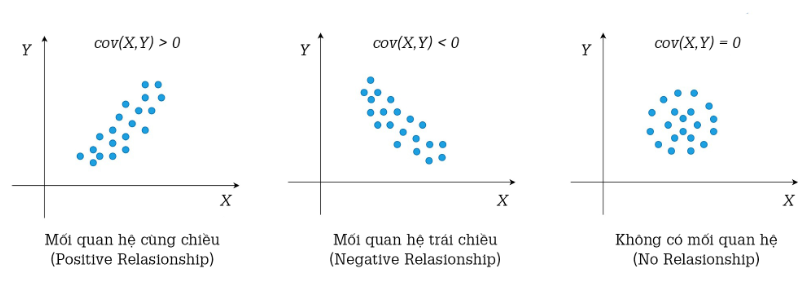
\includegraphics[width=\textwidth]{img/corvariance.png}
    \caption{Minh họa hiệp phương sai giữa hai biến ngẫu nhiên $X$ và $Y$.}
    \label{fig:covariance}
\end{figure}

\paragraph{}{Đồ thị trên minh họa ba trường hợp có thể xảy ra khi tính hiệp phương sai:}

\begin{itemize}
    \item Khi \(\text{cov}(X,Y) > 0\): Hai biến \(X\) và \(Y\) có quan hệ tuyến tính thuận, khi \(X\) tăng thì \(Y\) cũng tăng.
    \item Khi \(\text{cov}(X,Y) < 0\): Hai biến \(X\) và \(Y\) có quan hệ tuyến tính nghịch, khi \(X\) tăng thì \(Y\) giảm và ngược lại.
    \item Khi \(\text{cov}(X,Y) = 0\): Hai biến \(X\) và \(Y\) không có mối quan hệ tuyến tính với nhau.
\end{itemize}
\subsection{Ma trận hiệp phương sai (Covariance matrix)}

\paragraph{}{\textbf{Ma trận hiệp phương sai} là một ma trận vuông chứa các hiệp phương sai giữa các biến trong một tập dữ liệu. Nếu một tập dữ liệu có \( p \) biến ngẫu nhiên \( X_1, X_2, \dots, X_p \), thì ma trận hiệp phương sai \( \Sigma \) có dạng:}

\[
\Sigma =
\begin{bmatrix}
\text{Var}(X_1) & \text{Cov}(X_1, X_2) & \dots & \text{Cov}(X_1, X_p) \\
\text{Cov}(X_2, X_1) & \text{Var}(X_2) & \dots & \text{Cov}(X_2, X_p) \\
\vdots & \vdots & \ddots & \vdots \\
\text{Cov}(X_p, X_1) & \text{Cov}(X_p, X_2) & \dots & \text{Var}(X_p)
\end{bmatrix}
\]

Trong đó:
\begin{itemize}
\item \( \text{Var}(X_i) = \text{Cov}(X_i, X_i) \) là phương sai của biến \( X_i \).
\item \( \text{Cov}(X_i, X_j) \) là hiệp phương sai giữa hai biến \( X_i \) và \( X_j \).
\end{itemize}
\paragraph{}{\textbf{Công thức tổng quát:}
Giả sử có một tập dữ liệu với \( n \) quan sát và \( p \) biến ngẫu nhiên được biểu diễn dưới dạng ma trận \( X \) có kích thước \( n \times p \), với mỗi hàng là một quan sát và mỗi cột là một biến. Khi đó, ma trận hiệp phương sai được tính bằng công thức:}

\[
\Sigma = \frac{1}{n - 1} \sum_{i=1}^{n} (X_i - \bar{X})(X_i - \bar{X})^T
\]

Trong đó:
\begin{itemize}
\item \( X_i \) là vector giá trị của các biến tại quan sát thứ \( i \).
\item\( \bar{X} \) là vector trung bình của từng biến.
\end{itemize}
\paragraph{}{\textbf{Tính chất:}}
\begin{itemize}
    \item Ma trận hiệp phương sai là \textbf{ma trận đối xứng}.
    \item Đường chéo chứa phương sai của từng biến.
    \item Nếu các biến không có tương quan (độc lập tuyến tính), thì các phần tử ngoài đường chéo bằng 0.
\end{itemize}

\pagebreak

\section{PCA, EVR, CEVR}
\subsection{PCA}

\paragraph{Giới thiệu tổng quan:} 

\paragraph{}{Phân tích thành phần chính (PCA) là kỹ thuật giảm chiều, chuyển dữ liệu từ không gian ban đầu sang không gian mới với các thành phần chính không tương quan, giữ phần lớn phương sai. Hữu ích khi xử lý với các dữ liệu cao chiều.}

\paragraph{Các bước tính toán:}
\begin{enumerate}
  \item \textbf{Tính vector kì vọng của toàn bộ dữ liệu:}
    \[
        \mathbf{\overline{X}} = \frac{1}{N} \sum_{i=1}^{N} \vec{x_i}
    \]
    với $\vec{x_i}$ là sample thứ $i$ trong dữ liệu.
  \item \textbf{Chuẩn hóa dữ liệu:} Với ma trận dữ liệu $\mathbf{X} \in \mathbb{R}^{n \times p}$ ($n$ mẫu, $p$ biến), đưa về trọng tâm: 
      \[
      \mathbf{X}_{\text{centered}} = \mathbf{X} - \mathbf{\overline{X}},
      \]
      với $\mathbf{\overline{X}}$ là ma trận chứa các vector trung bình của các cột (đặc trưng). 
  \item \textbf{Tính ma trận hiệp phương sai:} 
      \[
      \mathbf{A} = \frac{1}{N} \mathbf{X}_{\text{centered}}^T \mathbf{X}_{\text{centered}},
      \]
      trong đó $\mathbf{A} \in \mathbb{R}^{d \times d}$ là ma trận hiệp phương sai, $N$ là số mẫu trong dữ liệu.
  \item \textbf{Phân tích giá trị riêng và vector riêng:} Tìm giá trị riêng $\lambda_i$ và vector riêng $\mathbf{v}_i$ của $\mathbf{A}$ sao cho:
      \[
      \mathbf{A} \mathbf{v}_i = \lambda_i \mathbf{v}_i, \quad i = 1, \dots, n.
      \]
      Các $\mathbf{v}_i$ là các hướng của thành phần chính với $\lambda_i$ là phương sai tương ứng.
  \item \textbf{Lựa chọn thành phần chính:} Sắp xếp $\lambda_i$ giảm dần và chọn số thành phần chính muốn giữ lại. Hoặc có thể tính tỷ lệ phương sai tích lũy như sau:
      \[
      \text{Tỷ lệ} = \frac{\sum_{i=1}^k \lambda_i}{\sum_{i=1}^n \lambda_i},
      \]
      rồi chọn $k$ thành phần sao cho tỷ lệ đạt 80-95\% tùy nhu cầu.
  \item \textbf{Chiếu dữ liệu:} Tạo ma trận $\mathbf{V}_k \in \mathbb{R}^{n \times k}$ từ $k$ vector riêng, chiếu dữ liệu:
      \[
      \mathbf{Z} = \mathbf{X}_{\text{centered}} \mathbf{V}_k,
      \]
      với $\mathbf{Z} \in \mathbb{R}^{n \times k}$ là dữ liệu trong không gian mới.
\end{enumerate}

\subsubsection*{Ý nghĩa:} 
\begin{itemize}
  \item \textbf{Thành phần chính (vector riêng):} Là các hướng $\mathbf{v}_i$ tối đa hóa phương sai. Các thành phần chính trực giao với nhau, giảm chiều mà giữ thông tin chính.
  \item \textbf{Trị riêng:} Cho biết mức độ quan trọng (explained variance) của mỗi thành phần chính. Trị riêng càng lớn thì phương sai theo hướng đó càng lớn, dẫn đến thành phần chính đó càng quan trọng.
\end{itemize}

\subsection{Explained variance ratio}

\paragraph{}{Explained Variance Ratio (EVR) cho biết tỷ lệ phương sai của dữ liệu được giải thích bởi mỗi thành phần chính. EVR giúp đánh giá mức độ quan trọng tương đối của từng thành phần.}

\textbf{Cách tính toán:} Với giá trị riêng $\lambda_i$ ($i = 1, \dots, n$) của ma trận hiệp phương sai $\mathbf{A}$, tỷ lệ phương sai được giải thích của thành phần chính thứ $i$ được tính bằng:
\[
\text{EVR}_i = \frac{\lambda_i}{\sum_{j=1}^n \lambda_j},
\]
trong đó $\sum_{j=1}^n \lambda_j$ là tổng phương sai của dữ liệu. Giá trị $\text{EVR}_i$ nằm trong khoảng $[0, 1]$ và thể hiện phần trăm phương sai mà thành phần chính thứ $i$ giải thích.

\textbf{Ý nghĩa:} Giá trị $\text{EVR}_i$ cao cho thấy thành phần chính thứ $i$ nắm giữ nhiều thông tin của dữ liệu gốc. Trong ứng dụng thực tế, các thành phần chính với $\text{EVR}_i$ lớn được ưu tiên giữ lại khi giảm chiều dữ liệu.

\subsection{Cumulative explained variance ratio}

\paragraph{}{Cumulative Explained Variance Ratio (CEVR) là tổng tích lũy của EVR, đo lường tổng phương sai được giữ lại khi sử dụng $k$ thành phần chính đầu tiên. CEVR là công cụ quan trọng để quyết định số lượng thành phần chính cần giữ lại.}

\textbf{Cách tính toán:} Với $k$ thành phần chính đầu tiên, tỷ lệ phương sai tích lũy được giải thích được tính bằng:
\[
\text{CEVR}_k = \sum_{i=1}^k \text{EVR}_i = \frac{\sum_{i=1}^k \lambda_i}{\sum_{j=1}^n \lambda_j},
\]
trong đó $\lambda_i$ là giá trị riêng tương ứng với thành phần chính thứ $i$ (đã sắp xếp giảm dần). Giá trị $\text{CEVR}_k$ tăng dần theo $k$ và nằm trong khoảng $[0, 1]$.

\textbf{Ý nghĩa:} 
\begin{itemize}
  \item Giá trị $\text{CEVR}_k$ cho biết tỷ lệ tổng thông tin dữ liệu được giữ lại khi sử dụng $k$ thành phần chính đầu tiên.
  \item Thông thường, người ta chọn số thành phần chính $k$ nhỏ nhất sao cho $\text{CEVR}_k \geq \alpha$, với $\alpha$ thường là 0.9 hoặc 0.95 tùy thuộc vào yêu cầu về mức độ bảo toàn thông tin.
\end{itemize}

\pagebreak 
\section{Thuật toán phân cụm}
\subsection{K-means clustering}

\paragraph{}{\textbf{K-Means} là một thuật toán phân cụm (clustering) phổ biến trong học máy, dùng để chia tập dữ liệu thành K cụm không giao nhau. Mỗi cụm được đại diện bởi một tâm (centroid). Mục tiêu của thuật toán là tối thiểu hóa tổng khoảng cách bình phương từ các điểm dữ liệu đến tâm cụm tương ứng.}

\paragraph{Thuật toán}
Cho dữ liệu $X = \{x_i\}_{i=1}^n, x_i \in \mathbb{R}^d$ và số cụm $k$:
\begin{enumerate}
  \item Khởi tạo ngẫu nhiên $k$ tâm cụm $\{\mu_j^{(0)}\}_{j=1}^k$.
  \item Lặp lại cho đến khi hội tụ (hoặc đạt số vòng lặp tối đa $T$):
    \begin{itemize}
      \item \textbf{Bước gán nhãn (Assignment step)}: Với mỗi điểm dữ liệu $x_i$, gán nó vào cụm $C_j$ có tâm $\mu_j^{(t)}$ gần nhất:
      \[
        c_i^{(t)} = \arg\min_{j \in \{1, \dots, k\}} \| x_i - \mu_j^{(t)} \|^2
      \]
      \item \textbf{Bước cập nhật tâm (Update step)}: Với mỗi cụm $C_j$, cập nhật lại tâm cụm $\mu_j^{(t+1)}$ là trung bình của tất cả các điểm dữ liệu được gán vào cụm đó:
      \[
        \mu_j^{(t+1)} = \frac{1}{|C_j^{(t)}|} \sum_{x_i \in C_j^{(t)}} x_i
      \]
      \item Nếu $\max_j \| \mu_j^{(t+1)} - \mu_j^{(t)} \| < \epsilon$ (một ngưỡng nhỏ) thì dừng.
    \end{itemize}
\end{enumerate}

% \begin{figure}[H]
%     \centering
%     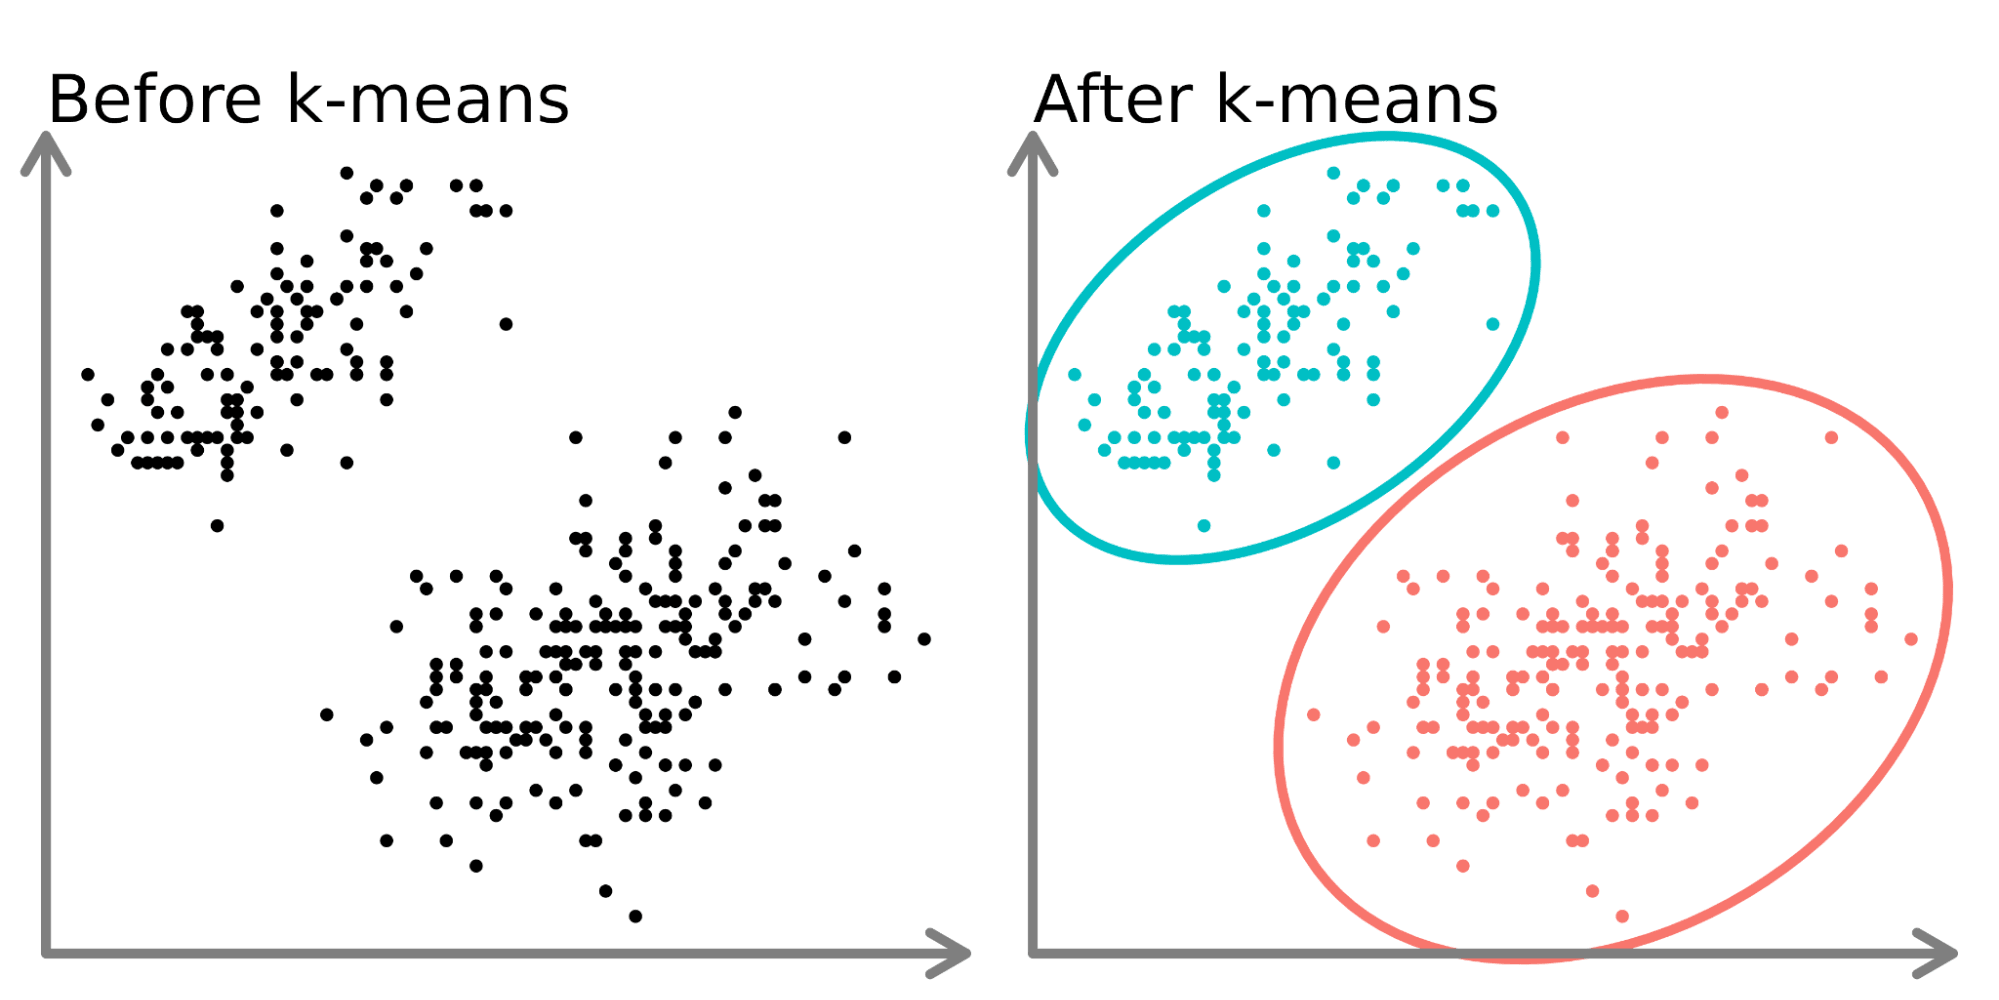
\includegraphics[width=0.8\linewidth]{k-means.png}
%     \caption{Minh họa thuật toán k-means}
% \end{figure}

\subsection{Gaussian Mixture Model}
\paragraph{}{Gaussian Mixture Model (GMM) là một mô hình xác suất dùng để biểu diễn sự phân bố dữ liệu như là sự kết hợp của nhiều phân phối chuẩn (Gaussian) đa biến. Nó giả định rằng dữ liệu được tạo ra từ một hỗn hợp của $K$ phân phối Gaussian, mỗi phân phối có bộ tham số (trung bình $\mu_k$, hiệp phương sai $\Sigma_k$) và trọng số $\pi_k$ riêng.}

\paragraph{}{Giả sử dữ liệu $\mathbf{x} \in \mathbb{R}^d$, GMM biểu diễn hàm mật độ xác suất như sau:}

\begin{equation}
p(\mathbf{x} | \Theta) = \sum_{k=1}^{K} \pi_k \cdot \mathcal{N}(\mathbf{x} | \mu_k, \Sigma_k)
\end{equation}

\paragraph{}{Trong đó $\Theta = \{\pi_k, \mu_k, \Sigma_k\}_{k=1}^K$ là tập hợp các tham số của mô hình.}

\begin{itemize}
  \item $K$ là số thành phần (số Gaussian).
  \item $\pi_k$ là trọng số trộn (mixing coefficient) của thành phần thứ $k$, với $\pi_k \ge 0$ và $\sum_{k=1}^{K} \pi_k = 1$.
  \item $\mathcal{N}(\mathbf{x} | \mu_k, \Sigma_k)$ là hàm mật độ xác suất của phân phối Gaussian đa biến thứ $k$:
  \begin{equation}
    \mathcal{N}(\mathbf{x} | \mu_k, \Sigma_k) = \frac{1}{(2\pi)^{d/2} |\Sigma_k|^{1/2}} \exp\left( -\frac{1}{2}(\mathbf{x} - \mu_k)^T \Sigma_k^{-1} (\mathbf{x} - \mu_k) \right)
  \end{equation}
\end{itemize}

\paragraph{}{Gaussian Mixture Model (GMM) thường được huấn luyện bằng thuật toán EM (Expectation-Maximization) để tìm các tham số $\Theta$ tối ưu hóa hàm hợp lý (likelihood) của dữ liệu.}

\paragraph{Thuật toán huấn luyện: EM (Expectation-Maximization)} {}
Thuật toán EM là một phương pháp lặp để tìm ước lượng hợp lý tối đa (MLE) của các tham số trong các mô hình xác suất thống kê có biến ẩn.
\begin{itemize}
  \item \textbf{Bước E (Expectation)}: Với các tham số hiện tại $\Theta^{(t)} = \{\pi_k^{(t)}, \mu_k^{(t)}, \Sigma_k^{(t)}\}$, tính toán xác suất hậu nghiệm (responsibility) $\gamma_{ik}$ rằng điểm dữ liệu $\mathbf{x}_i$ được tạo ra bởi thành phần Gaussian thứ $k$:
  \begin{equation}
    \gamma_{ik}^{(t)} = \frac{\pi_k^{(t)} \cdot \mathcal{N}(\mathbf{x}_i | \mu_k^{(t)}, \Sigma_k^{(t)})}{\sum_{j=1}^K \pi_j^{(t)} \cdot \mathcal{N}(\mathbf{x}_i | \mu_j^{(t)}, \Sigma_j^{(t)})}
  \end{equation}

  \item \textbf{Bước M (Maximization)}: Cập nhật các tham số mô hình $\Theta^{(t+1)}$ dựa trên các xác suất hậu nghiệm $\gamma_{ik}^{(t)}$ đã tính ở bước E:
  \begin{align}
    N_k^{(t+1)} &= \sum_{i=1}^{N} \gamma_{ik}^{(t)} \quad (\text{số điểm hiệu dụng cho cụm } k) \\
    \pi_k^{(t+1)} &= \frac{N_k^{(t+1)}}{N} \\
    \mu_k^{(t+1)} &= \frac{1}{N_k^{(t+1)}} \sum_{i=1}^{N} \gamma_{ik}^{(t)} \cdot \mathbf{x}_i \\
    \Sigma_k^{(t+1)} &= \frac{1}{N_k^{(t+1)}} \sum_{i=1}^{N} \gamma_{ik}^{(t)} (\mathbf{x}_i - \mu_k^{(t+1)})(\mathbf{x}_i - \mu_k^{(t+1)})^T
  \end{align}
  Trong đó $N$ là tổng số điểm dữ liệu.
\end{itemize}

\paragraph{}{Lặp lại các bước E và M cho đến khi hàm log-likelihood hội tụ hoặc đạt số vòng lặp tối đa.}

\pagebreak
\newpage
\section{Các phương pháp đánh giá mô hình}

\paragraph{}{Kết quả dự đoán của mô hình phân loại (Classification) là các nhãn rời rạc, chúng ta cần các chỉ số đánh giá (evaluation metrics) để đo lường mức độ chính xác và hiệu quả trong việc phân loại các mẫu vào đúng nhãn. Các chỉ số phổ biến bao gồm \textbf{Accuracy}, \textbf{Precision}, \textbf{Recall} và \textbf{F1-score}. Mỗi chỉ số phản ánh một khía cạnh khác nhau của hiệu suất mô hình. Ngoài ra, \textbf{Confusion Matrix} cũng là một công cụ quan trọng giúp trực quan hóa chi tiết số lượng các dự đoán đúng và sai theo từng lớp, đặc biệt hữu ích trong các bài toán phân loại nhiều lớp hoặc mất cân bằng lớp.}

\paragraph{Các ký hiệu sau được sử dụng trong các công thức đánh giá}

\begin{itemize}
  \item \textbf{TP} (True Positive): Dự đoán đúng mẫu thuộc lớp dương tính (positive class).
  \item \textbf{TN} (True Negative): Dự đoán đúng mẫu thuộc lớp âm tính (negative class).
  \item \textbf{FP} (False Positive): Dự đoán sai, mô hình dự đoán dương tính nhưng thực tế là âm tính.
  \item \textbf{FN} (False Negative): Dự đoán sai, mô hình dự đoán âm tính nhưng thực tế là dương tính.
\end{itemize}

\subsection{Accuracy}

\paragraph{}{Accuracy đo lường tỷ lệ các dự đoán chính xác trên tổng thể.Công thức của Accuracy: }

\[
\text{Accuracy} = \frac{TP + TN}{TP + TN + FP + FN}
\]



\subsection{Precision}
\paragraph{}{Precision đo lường tỷ lệ dự báo chính xác các trường hợp dương tính (positive) trên tổng số trường hợp mà mô hình dự đoán là dương tính. Công thức của Precision như sau:}

\[
\text{Precision} = \frac{TP}{TP + FP}
\]

\subsection{Recall}

\paragraph{}{Recall đo lường tỷ lệ dự báo chính xác các trường hợp positive trên toàn bộ các mẫu thuộc nhóm Positive.Công thức của recall như sau:}

\[
\text{Recall} = \frac{TP}{TP + FN}
\]

\subsection{F1-Score}

\paragraph{}{F1-score là chỉ số tổng hợp dùng để cân bằng giữa Precision và Recall. F1-score đặc biệt hữu ích khi cần sự cân bằng giữa độ chính xác và độ bao phủ trong các mô hình phân loại. Công thức của F1-score như sau:}

\[
\text{F1-score} = 2 \cdot \frac{\text{Precision} \cdot \text{Recall}}{\text{Precision} + \text{Recall}}
\]

\subsection{Confusion Matrix}

\paragraph{}{Confusion Matrix minh họa số lượng dự đoán đúng/sai cho từng lớp. Với bài toán phân loại nhị phân, ma trận có dạng:}

\[
\begin{array}{|c|c|c|}
\hline
\multirow{2}{*}{\textbf{Actual}} & \multicolumn{2}{c|}{\textbf{Predicted}} \\
\cline{2-3}
& \text{Negative (No)} & \text{Positive (Yes)} \\
\hline
\text{Negative (No)} & \text{TN} & \text{FP} \\
\hline
\text{Positive (Yes)} & \text{FN} & \text{TP} \\
\hline
\end{array}
\]


Từ ma trận này, ta có thể dễ dàng tính được các chỉ số như Accuracy, Precision, Recall và F1-score.

\pagebreak %DONE
\newpage
\section{Bộ dữ liệu hoa Iris}

\subsection{Tải dữ liệu và tổng quan về dữ liệu} 
\paragraph{}{\textbf{Bộ dữ liệu hoa Iris} hay bộ dữ liệu Iris của Fisher là một bộ dữ liệu đa biến nổi tiếng và được nhà thống kê và nhà sinh vật học người Anh Ronald Fisher sử dụng trong bài báo năm 1936 của ông: "The use of multiple measurements in taxonomic problems". \cite{fisher1936use}}
\paragraph{}{Bộ dữ liệu được cung cấp bởi thư viện scikit-learn.}
\begin{itemize}
    \item \textbf{150 dòng}: thông tin về 150 mẫu hoa Iris, thuộc 3 loại: Setosa, Versicolour và Virginica.
    \item \textbf{5 cột}: thông tin về kích thước hoa Iris và loại hoa, trong đó:
    \begin{itemize}
        \item \texttt{Sepal Length}: độ dài đài hoa
        \item \texttt{Sepal Width}: độ rộng đài hoa
        \item \texttt{Petal Length}: độ dài cánh hoa
        \item \texttt{Petal Width}: độ rộng cánh hoa
        \item \texttt{Target}: loại hoa (mã hóa dưới dạng 0, 1, 2)
    \end{itemize}
\end{itemize}

\begin{figure}[H]
    \centering
    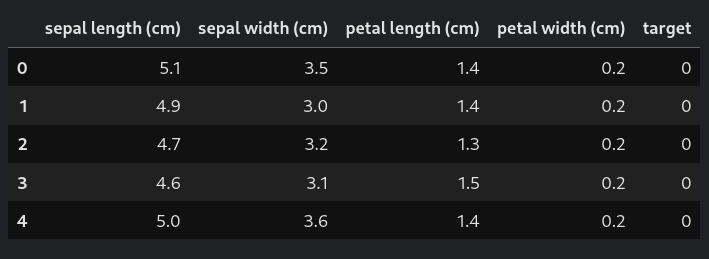
\includegraphics[width=0.8\linewidth]{img/iris_head.png}
    \caption{Các dòng đầu tiên trong bộ dữ liệu Iris}
    \label{fig:iris_head}
\end{figure}

\subsection{Phân tích và dự đoán loại hoa Iris}
\paragraph{}{Sau khi dùng chuẩn hóa \textbf{Z-score} và phân tích thành phần chính (\textbf{PCA}) trên bộ dữ liệu Iris, chúng ta thu được:}
\begin{itemize}
    \item \textbf{EVR} (Explained variance ratio) được nắm giữ bởi thành phần chính thứ nhất (PC1) và thành phần chính thứ hai (PC2) lần lượt là \texttt{0.97343527}  và \texttt{0.01707156}.
    \item \textbf{CEVR} (Cumulative explained variance ratio) của PC1 và PC2 là \texttt{0.990506835254475}.
\end{itemize}

\paragraph{}{Điều này thể hiện chỉ với hai thành phần chính đầu tiên, 99\% tỉ lệ phương sai của dữ liệu được nắm giữ bởi PC1 và PC2.}

\paragraph{}{Tiếp theo, ta áp dụng thuật toán k-means với k = 3 và thu được kết quả sau:}

\begin{figure}[H]
    \centering
    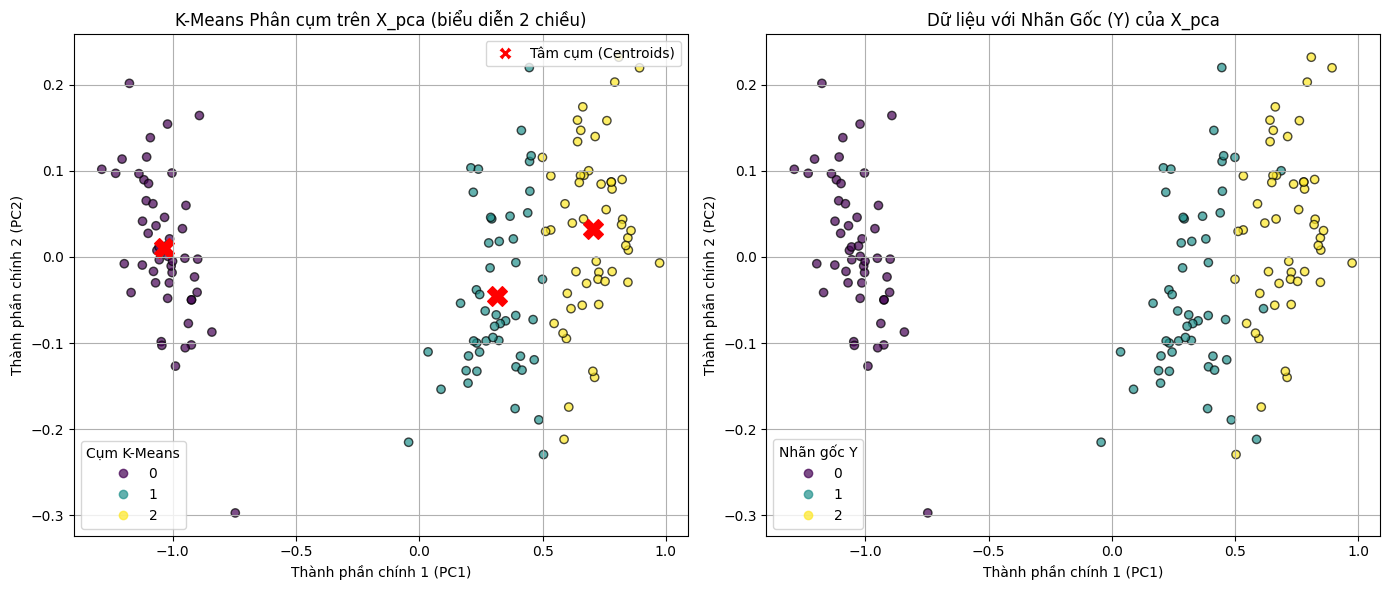
\includegraphics[width=1\linewidth]{img/iris_plot.png}
    \caption{Kết quả phân cụm trên bộ dữ liệu Iris}
    \label{fig:iris_plot}
\end{figure}

\begin{itemize}
    \item Kết quả phân cụm chính xác tới \textbf{96\%} sau khi nối nhãn với cụm phù hợp (bằng thuật toán Hungary).
    \item Ba cụm điểm dữ liệu được phân biệt rõ ràng trên mặt phẳng 2 chiều và có thể nhận biết bằng mắt thường.
\end{itemize}

\pagebreak %DONE
\section{Bộ dữ liệu ABIDE II}

\subsection{Tải dữ liệu và tổng quan về dữ liệu}
\paragraph{}{Bộ cơ sở dữ liệu \textbf{ABIDE II} \cite{DiMartino2017abideII} được giới thiệu ở NeuroHackademy 2020 bới giáo sư Tal Yarkoni.
Bộ dữ liệu đã được thay đổi một ít để phù hợp với lab này, cụ thể sẽ là phân cụm bệnh nhân có bị ung thư (cancer) hay không (normal).}

\paragraph{}{Dữ liệu được cung cấp trong file \texttt{ABIDE2(updated).csv}, trong đó:}

\begin{itemize}
    \item Số dòng: 1004. Trong đó có 463 bệnh nhân bị ung thư và 541 bệnh
nhân không bị ung thư.
    \item  Số cột: 1444
    \begin{itemize}
    \item \texttt{Unnamed: 0}: Chỉ số dòng (index)
    \item \texttt{Site}: Nơi thu thập dữ liệu (ví dụ: \texttt{ABIDEII-KKI\_1})
    \item \texttt{Subject}: ID của đối tượng nghiên cứu
    \item \texttt{Age}: Tuổi của đối tượng
    \item Các chỉ số còn lại là dữ liệu đặc trưng về não bộ
    \begin{itemize}
        \item Tiền tố \texttt{\texttt{fsArea\_}} (FreeSurfer Area): Diện tích bề mặt của một vùng vỏ não (mm\textsuperscript{2}).
        \item Tiền tố \texttt{\texttt{fsVol\_}} (FreeSurfer Volume): Thể tích của một vùng vỏ não hoặc cấu trúc dưới vỏ não (mm\textsuperscript{3}). 
        \item Tiền tố \texttt{\texttt{fsLGI\_}} (FreeSurfer Local Gyrification Index): Là một thước đo mức độ gấp cuộn của vỏ não tại một vùng cụ thể. Chỉ số này phản ánh mức độ phức tạp của các nếp cuộn não (gyri) và rãnh não (sulci) ở quy mô cục bộ.
        \item Tiền tố \texttt{\texttt{fsCT\_}} (FreeSurfer Cortical Thickness): Độ dày của vỏ não (mm).
 \newline
 \texttt{Chữ cái \texttt{L} và \texttt{R}} trong tên cột: biểu thị bán cầu não trái (\textit{Left}) hoặc phải (\textit{Right}).

   \item \textbf{ROI}: \textit{Region of Interest} – Vùng quan tâm trong nghiên cứu ảnh não.
  
    \end{itemize}
\item \texttt{Group}. Cột này gồm  2 giá trị là: \texttt{Cancer} và \texttt{Normal}.
    \end{itemize}
\end{itemize}

\subsection{Phân tích và dự đoán bệnh nhân}

\paragraph{}{Sau khi dùng chuẩn hóa \textbf{Z-score} và phân tích thành phần chính (\textbf{PCA}) trên bộ dữ liệu ABIDE II, chúng ta thu được:}
\begin{itemize}
    \item \textbf{EVR} (Explained variance ratio) được nắm giữ bởi thành phần chính thứ nhất (PC1) và thành phần chính thứ hai (PC2) lần lượt là \texttt{0.08663063}  và \texttt{0.06472462}.
    \item \textbf{CEVR} (Cumulative explained variance ratio) của PC1 và PC2 là \texttt{0.15135524985487855}.
    \item \textbf{CEVR} của 200 thành phần chính đầu tiên thì đạt gần tới \texttt{0.95}.
\end{itemize}

\begin{figure}[H]
    \centering
    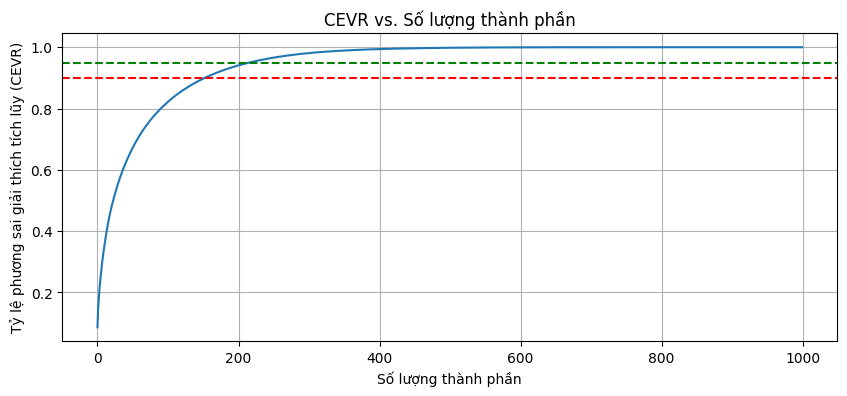
\includegraphics[width=1\linewidth]{img/all_cevr.png}
    \caption{CEVR tương ứng với số lượng thành phần chính}
    \label{fig:all_cevr}
\end{figure}

\paragraph{}{Chúng tôi chọn \texttt{n-components} = 2 cho PCA vì khả năng diễn giải tốt trên mặt phẳng hai chiều và kết quả chấp nhận được với hai thuật toán phân cụm.}

\subsection{Sử dụng thuật toán K-Means}

\paragraph{}{Tiếp theo, ta áp dụng thuật toán k-means với k = 2 và thu được kết quả sau:}

\begin{figure}[H]
    \centering
    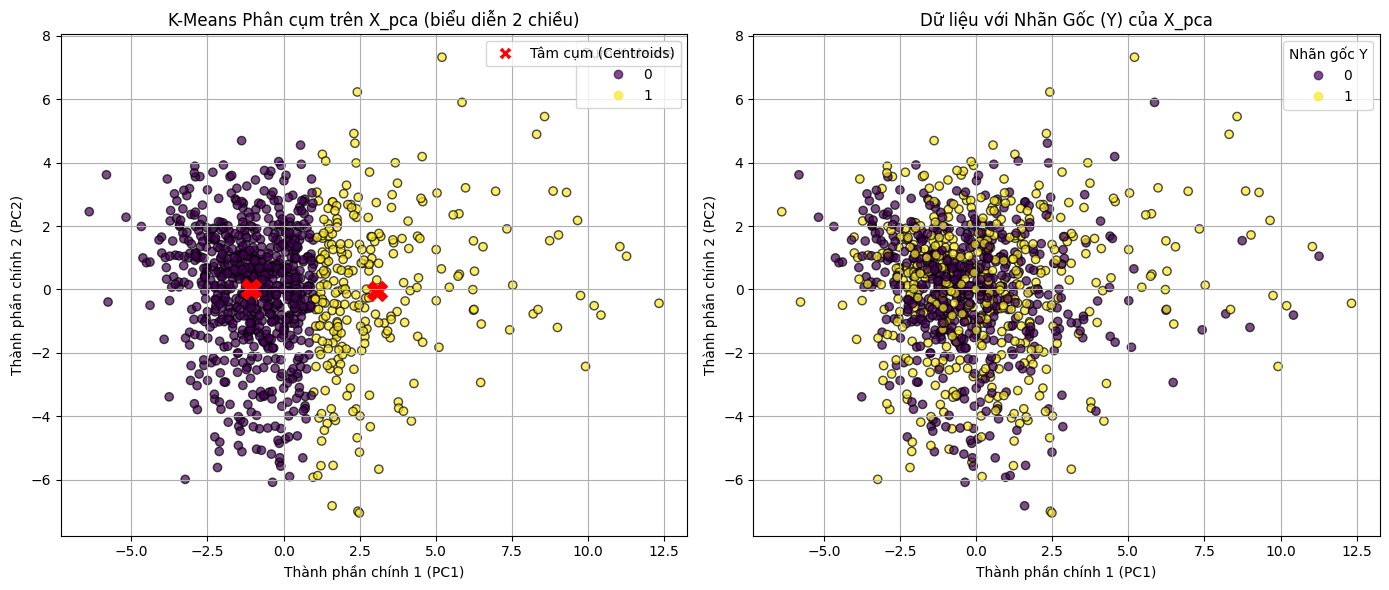
\includegraphics[width=1\linewidth]{img/abideii_plot.png}
    \caption{Kết quả phân cụm bằng KMeans trên bộ dữ liệu ABIDE II}
    \label{fig:abideii_plot}
\end{figure}

\begin{itemize}
    \item Kết quả phân cụm chính xác \textbf{58.1\%} sau khi nối nhãn với cụm phù hợp (bằng thuật toán Hungary). \texttt{Accuracy:} \texttt{0.581}. \texttt{Recall:} \texttt{0.307}. \texttt{Precision:} \texttt{0.587}.  \texttt{F1-score:} \texttt{0.403}. 
    \item Hai cụm dữ liệu thật trên mặt phẳng hai chiều không thể phân biệt rõ được. Tuy nhiên nhãn \texttt{Normal} so với nhãn \texttt{Cancer} có mật độ cao hơn ở trung tâm.
\end{itemize}

\subsection{Sử dụng thuật toán GMM}

\begin{figure}[H]
    \centering
    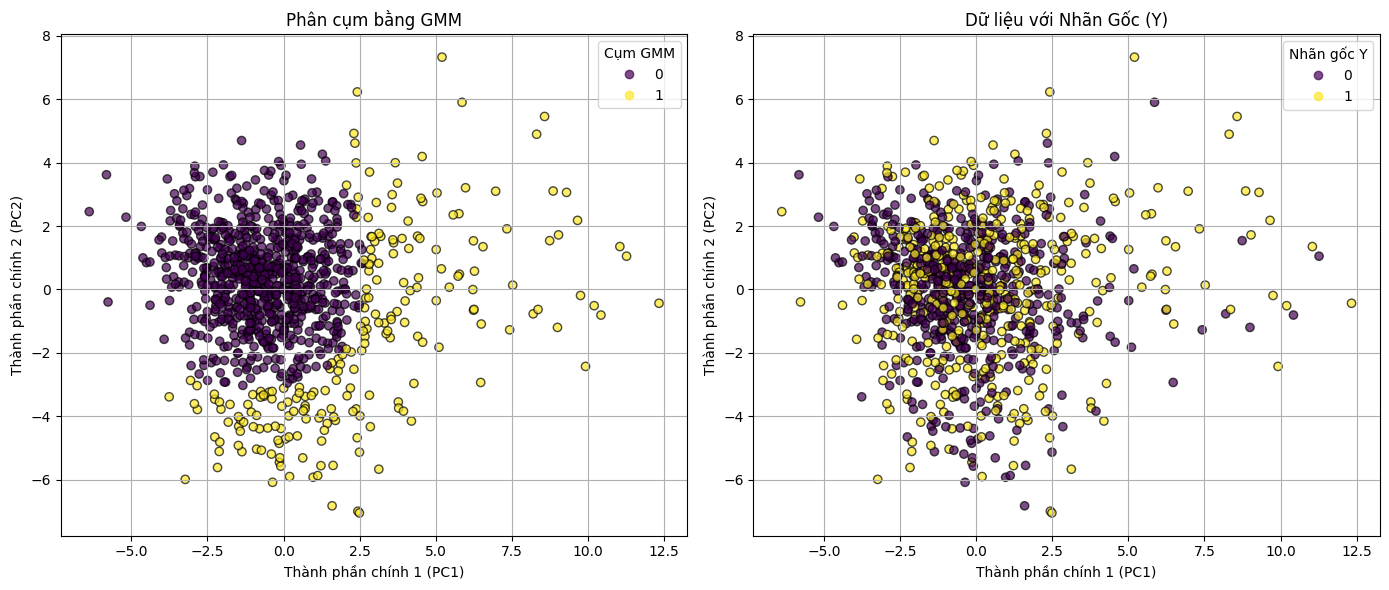
\includegraphics[width=1\linewidth]{img/abideii_plot_gmm.png}
    \caption{Kết quả phân cụm bằng GMM trên bộ dữ liệu ABIDE II}
    \label{fig:abideii_plot_gmm}
\end{figure}

\begin{itemize}
    \item Kết quả phân cụm chính xác \textbf{56.7\%} sau khi nối nhãn với cụm phù hợp (bằng thuật toán Hungary). \texttt{Accuracy:} \texttt{0.567}. \texttt{Recall:} \texttt{0.266}. \texttt{Precision:} \texttt{0.564}.  \texttt{F1-score:} \texttt{0.361}. 
\end{itemize}

\subsection{Nhận xét kết quả phân cụm}
\paragraph{}{Khi áp dụng cả hai thuật toán K-Means và GMM lên bộ dữ liệu ABIDE II (sau khi giảm chiều bằng PCA xuống còn 2 thành phần chính), chúng ta có thể đưa ra một số nhận xét sau:}

\begin{itemize}
    \item Với giá trị F1-score khá thấp nên cả hai thuật toán K-Means và GMM đều cho thấy hiệu suất phân cụm chưa cao khi đánh giá dựa trên nhãn thực tế, với độ chính xác (Accuracy) chỉ nhỉnh hơn một chút so với mức ngẫu nhiên. Điều này cho thấy rằng cấu trúc tự nhiên của dữ liệu không dễ dàng tách thành hai cụm tương ứng hoàn toàn với hai nhóm Cancel và Normal.
    \item Đặc biệt, chỉ số Recall ở cả hai thuật toán đều khá thấp, cho thấy mô hình gặp khó khăn trong việc xác định đúng các trường hợp thuộc nhóm "Cancer" (nếu giả định "Cancer" là lớp positive). Precision tuy cao hơn Recall nhưng vẫn ở mức trung bình.
    \item Quan sát biểu đồ trực quan (Hình 5 và Hình 6), cả K-Means và GMM đều cho thấy sự chồng lấn đáng kể giữa các cụm dữ liệu. Không có một ranh giới rõ ràng nào có thể tách biệt hoàn toàn hai nhóm bệnh nhân. Điều này lý giải tại sao độ chính xác đạt được không cao. Mặc dù có ghi nhận rằng nhãn "Normal" có mật độ cao hơn ở trung tâm, sự phân bố tổng thể vẫn rất phức tạp.
\end{itemize}

\pagebreak %DONE
\newpage
\section{Kết luận}

\subsection{Bộ dữ liệu hoa Iris}

\paragraph{}{Sử dụng phương pháp \textbf{PCA} và thuật toán \textbf{k-means} cho kết quả phân cụm chính xác đến \textbf{96\%} trên bộ dữ liệu hoa Iris. Điều đó cho thấy chỉ cần PCA và k-means - một thuật toán học không giám sát là đủ để phân loại trên bộ dữ liệu hoa Iris.}

\subsection{Bộ dữ liệu ABIDE II}

\paragraph{}{Sử dụng phương pháp \textbf{PCA} và thuật toán \textbf{k-means} cho kết quả phân cụm chính xác \textbf{58.1\%} trên bộ dữ liệu ABIDE II (đã qua chỉnh sửa). Các thông số khác: \texttt{Recall:} \texttt{0.307}, \texttt{Precision:} \texttt{0.587},  \texttt{F1-score:} \texttt{0.403}.}

\paragraph{}{Sử dụng phương pháp \textbf{PCA} và thuật toán \textbf{GMM} cho kết quả phân cụm chính xác \textbf{56.7\%} trên bộ dữ liệu ABIDE II (đã qua chỉnh sửa). Các thông số khác: \texttt{Recall:} \texttt{0.266}, \texttt{Precision:} \texttt{0.564},  \texttt{F1-score:} \texttt{0.361}.}

\paragraph{}{Qua các độ đo trên, đặc biệt là \texttt{Accuracy:} \texttt{0.576}, ta thấy chỉ dùng các phương pháp biến đổi số học như PCA và mô hình học máy học không giám sát như K-Means và GMM khó phân loại được bệnh nhân ung thư (cancer) và người bình thường (normal) trên bộ dữ liệu ABIDE II (đã qua chỉnh sửa).}

\paragraph{}{Nếu được sử dụng các kĩ thuật học sâu (deep learning), chúng tôi đề xuất dùng Generative Adversarial Network (GAN) và Graph Convolution Network (GCN) \cite{huynh2024use} cùng với học có giám sát để có thể cải thiện hơn trong tác vụ dự đoán người bệnh.}

\pagebreak % 0

\newpage
\bibliographystyle{unsrt}
\bibliography{ref/ref}

\appendix
\section{Phụ lục}
\begin{itemize}
\item Template này \textbf{không phải} là template chính thức của Khoa Công nghệ thông tin - Trường Đại học Khoa học Tự nhiên.
\item Các hình ảnh, bảng biểu, thuật toán trong template chỉ mang tính chất ví dụ.
\item Nhóm tác giả phân phối \textbf{miễn phí} template này \href{https://github.com/khongsomeo/hcmus-unofficial-report-template}{trên GitHub} và \href{https://www.overleaf.com/latex/templates/hcmus-report-template/zyrhmsxynwqs}{trên Overleaf} với \href{https://github.com/khongsomeo/hcmus-unofficial-report-template/blob/main/LICENSE}{Giấy phép GNU General Public License v3.0}. Nhóm tác giả không chịu trách nhiệm với các bản phân phối không nằm trong hai kênh phân phối chính thức nêu trên.
\end{itemize}


\end{document}